\chapter{Demonstration}
\label{demonstration}
In the previous chapters, Dynamic OpenCL was presented as a library, being included for single jobs or a predetermined amount of mixed workloads. Hence, it only acted on behalf of the calling code and was never used in a truly shared environment where multiple users could submit their respective workloads. Therefore this chapter showcases a developed software that allows users to compute jobs through a web interface with the option to adjust the computational capabilities during execution. For this, the software is connected to the EC2 and can therefore operate a hybrid cloud. In this demonstrated use case users can not submit their own programs but can choose from a variety of already implemented algorithms that can process supplied input. For instance, users can provide data for two matrices, which shall be multiplied, although the executing algorithm is already given by the system.

\section{Architecture}

\begin{figure}[!htb]
	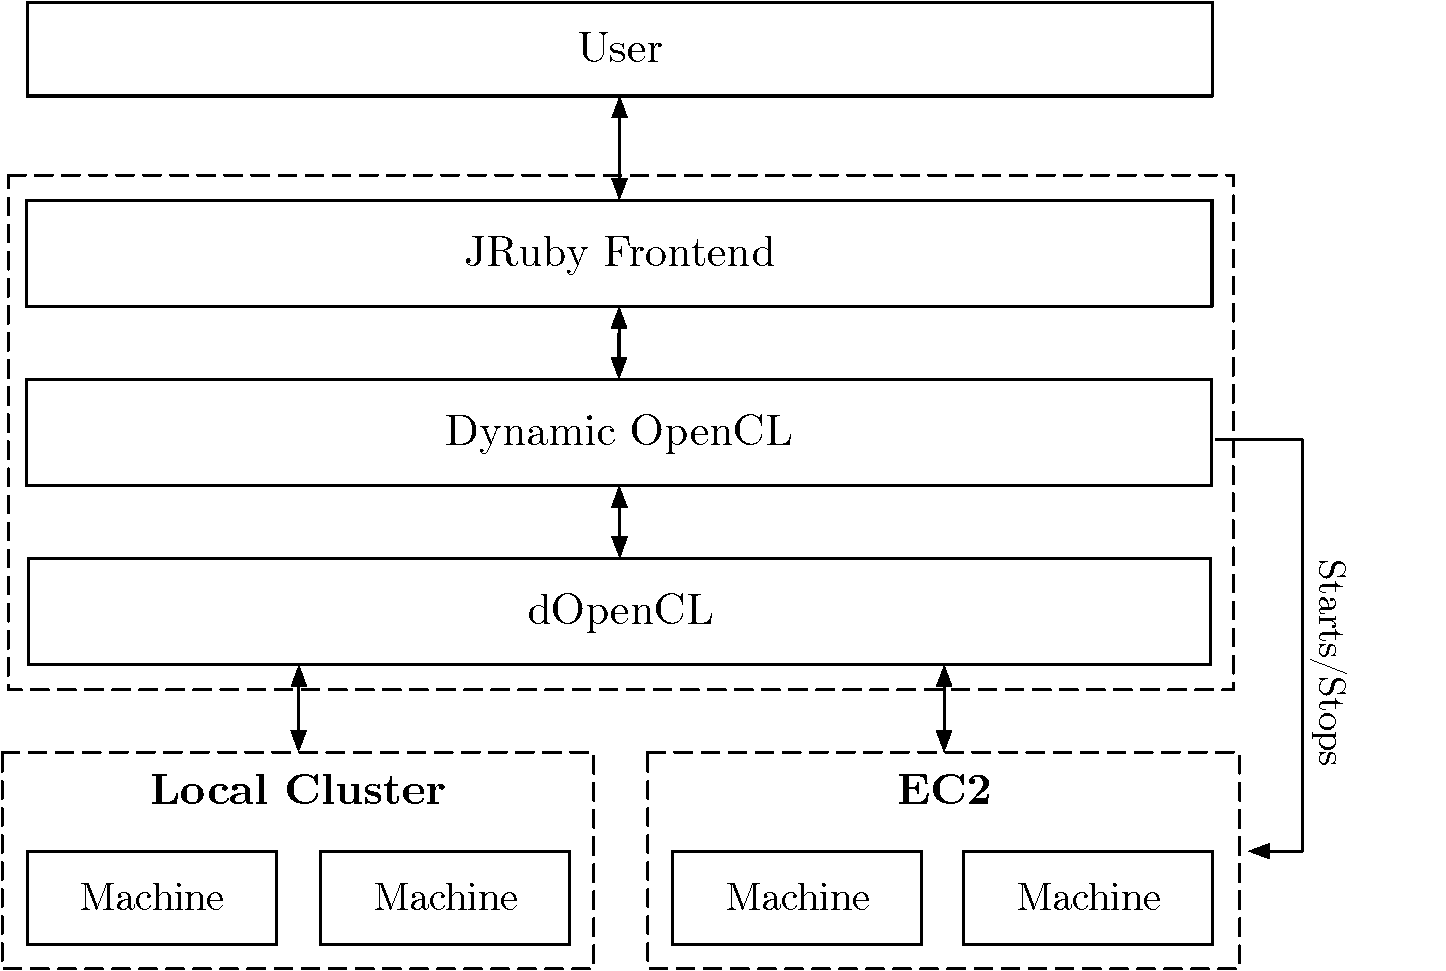
\includegraphics[width=0.8\textwidth]{drawings/demo_architecture.pdf}
	\centering
	\caption{Demo Architecture}
	\label{img:demo_architecture}
\end{figure}
The architecture of the developed system is shown in figure \ref{img:demo_architecture}. Users can access the service via a web frontend on the management node. As Dynamic OpenCL is written in Java and hence distributed as a \textit{Java Archive} file, the web frontend must run in a JVM. In this case, the web server was written in Ruby and runs as a JRuby application, which executes the Ruby code in a JVM.

The website offers user interfaces for submitting jobs, reviewing progress and changing the cluster configuration. It mainly communicates with Dynamic OpenCL, passing execution calls to it as well as retrieving necessary information. Dynamic OpenCL then is connected to the local dOpenCL installation that carries out the actual computations either on local hardware or cloud resources. The web frontend also allows users to dynamically book cloud instances. These bookings are carried out by Dynamic OpenCL through the AWS SDK, which communicates with the EC2 cloud.
\section{User Interface}

The system gives users the possibility to manually book or disband cloud resources based on their requirements and current resource utilization. Figure \ref{img:machine_order} shows the form that provides these functions. The currently available cloud resources are listed and can be removed by pressing a button in the table. This view ignores local resources as those can not be simply disbanded and therefore only lists already running cloud instances. Below the table is a drop-down list with all available EC2 instance types, which is used to specify the resources to book.

\begin{figure}[!htb]
	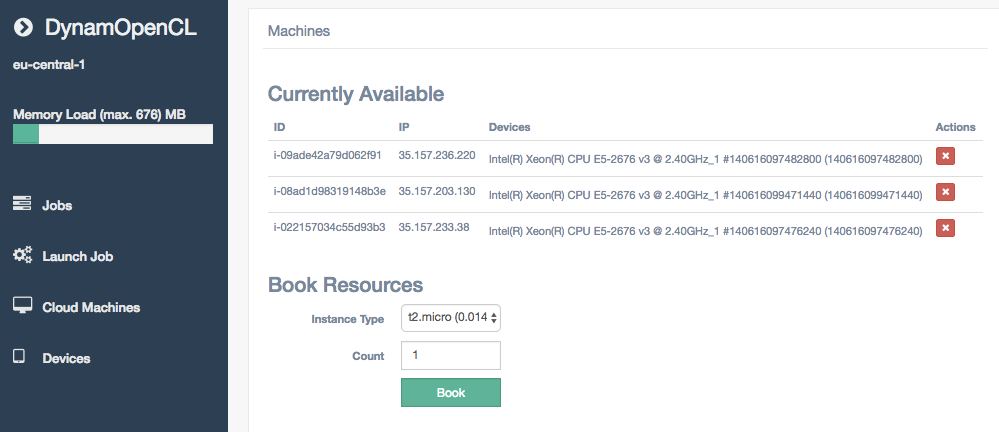
\includegraphics[width=1\textwidth]{screenshots/machine_order.png}
	\centering
	\caption{Ordering Cloud Resources}
	\label{img:machine_order}
\end{figure}

In figure \ref{img:available_devices} the device listing is portrayed, including all devices that are available through dOpenCL. The list contains local resources as well as the cloud resources, which are accordingly marked. It also displays the names of the devices with the corresponding clock speeds and number of cores.

\begin{figure}[!htb]
	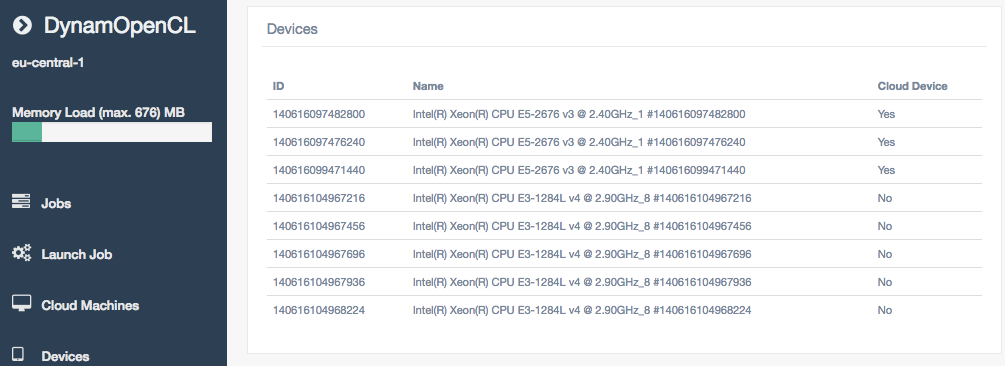
\includegraphics[width=1\textwidth]{screenshots/available_devices.png}
	\centering
	\caption{List of available Devices}
	\label{img:available_devices}
\end{figure}

Submitted jobs are listed in an overview screen, which includes progress information like the number of finished parts and how many parts are currently being computed. By taking historic performance measurements an estimate for the remaining time until completion can be given. A screenshot of this view can be seen in figure \ref{img:job_overview}. Pressing the \textit{Details} button for a job leads to a more fine-grained view about the historic performance of the various devices.

\begin{figure}[!htb]
	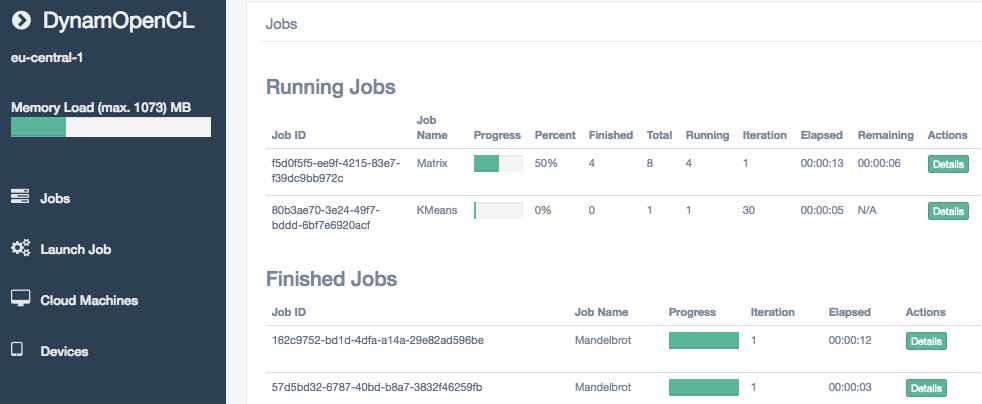
\includegraphics[width=1\textwidth]{screenshots/job_overview.png}
	\centering
	\caption{Job Overview}
	\label{img:job_overview}
\end{figure}

The details page of a job, which is displayed in figure \ref{img:job_details}, includes valuable information about the historic performance of every device that has participated in the computation of the job. It shows how many parts each device has finished as well as an average runtime per partial with its standard deviation. On the bottom of the page, the active devices currently computing partials for this job are visible.

\begin{figure}[!htb]
	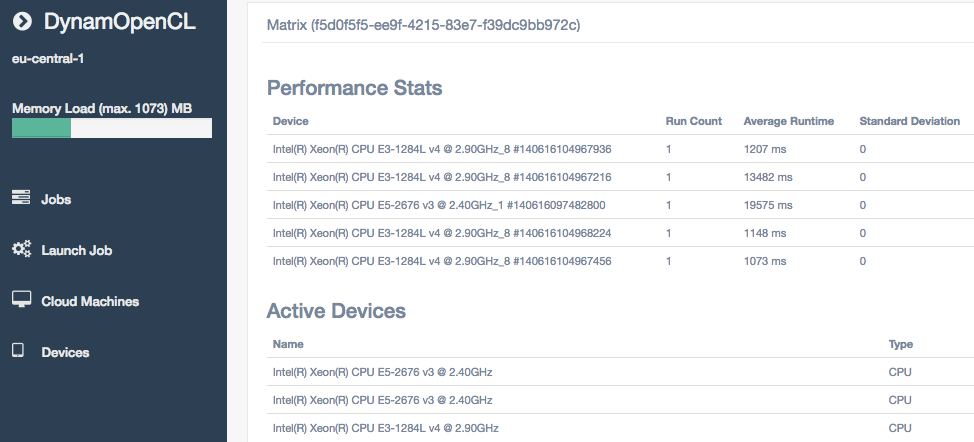
\includegraphics[width=1\textwidth]{screenshots/job_details.png}
	\centering
	\caption{Job Performance Stats}
	\label{img:job_details}
\end{figure}
